%=====================================================================
%  MMSS Graph Theory  .  Daily Report + Solutions Template
%
%  How to use:
%    1. Rename per session, e.g. mmss_graphtheory_0722.tex
%    2. Edit the two \newcommand lines just below (team + date).
%    3. Edit the FRONTMATTER block inside the document.
%    4. Write problems inside the enumerate. Use the graph toolkit.
%
%  Graph toolkit cheat sheet (all go INSIDE a graphfig / tikzpicture):
%    \gcycle{n}{radius}{prefix}      n vertices on a circle, joined as a cycle
%    \gcyclen{n}{radius}{prefix}     same, but vertices numbered 1..n
%    \gcomplete{n}{radius}{prefix}   complete graph K_n on a circle
%    \gbipartite{m}{n}{gap}          complete bipartite K_{m,n}
%                                      handles: left bl1..blm, right br1..brn
%    \gpath{n}{spacing}{prefix}      path on n vertices, left to right
%    \gpeterson                      the Petersen graph
%                                      handles: outer po0..po4, inner pin0..pin4
%    \gcube{n}                       n x n x n cube in oblique 2D projection
%    \gpancake{n}{radius}            pancake graph P_n: all n! permutations on a
%                                      circle, joined by prefix-reversal. Nodes
%                                      named p<perm>, e.g. p1234. Practical n=3,4
%                                      (n=5 is 120 nodes). Each node auto-labelled.
%  Named handles stay live in the picture, so after a call you can add e.g.
%    \draw[edge,densely dashed] (po0)--(pin2);   or   \node[hv] at (bl1){};
%  Vertex styles:  v (filled dot)  .  ov (open ring)  .  hv (highlighted hub)
%  Figure wrapper:  \begin{graphfig}[scale]{Label} ... \end{graphfig}
%    {Label} text -> titled [Graph Label];  {NUM} -> auto 1,2,3;  {} -> bare/inline
%=====================================================================
\documentclass[11pt]{article}

\usepackage[margin=1in,headheight=30pt,headsep=16pt]{geometry}
\usepackage{amsmath,amssymb,amsfonts,amsthm}
\usepackage{enumitem}
\usepackage{fancyhdr}
\usepackage{graphicx}
\usepackage{tikz}
\usepackage{xcolor}
\definecolor{amethyst}{rgb}{0.6, 0.4, 0.8}
\usetikzlibrary{arrows.meta,calc}

\newcommand{\teamname}{Group Name}
\newcommand{\reportdate}{\today}

\pagestyle{fancy}
\fancyhf{}
\renewcommand{\headrulewidth}{0.4pt}
\renewcommand{\footrulewidth}{0pt}
\fancyhead[L]{\raisebox{2pt}{\small\textsc{\teamname}}}
\fancyhead[R]{
\includegraphics[height=10pt]{logo.png}}
\fancyfoot[C]{\small\thepage}

\fancypagestyle{firstpage}{
  \fancyhf{}
  \renewcommand{\headrulewidth}{0pt}
  \fancyfoot[C]{\small\thepage}
}

\setlength{\parindent}{0pt}
\setlength{\parskip}{6pt}

\newcommand{\divider}{\begin{center}\rule{0.6\textwidth}{0.4pt}\end{center}}

\newtheoremstyle{solstyle}{6pt}{6pt}{}{}{\bfseries}{.}{ }{}
\theoremstyle{solstyle}
\newtheorem*{solution}{Solution}

\newcommand{\WLoG}{WLoG}
\newcommand{\Cn}[1]{C_{#1}}
\newcommand{\Kn}[1]{K_{#1}}
\newcommand{\Kt}[2]{K_{#1,#2}}

\tikzset{
  v/.style ={circle, fill=black, inner sep=1.6pt},
  ov/.style={circle, draw=black, fill=white, line width=0.6pt, inner sep=1.6pt},
  hv/.style={circle, fill=black!55, draw=black, line width=0.6pt, inner sep=2.6pt},
  edge/.style={line width=0.6pt},
}

\newcommand{\gcycle}[3]{
  \foreach \gi in {1,...,#1}{\node[v] (#3\gi) at ({90-(\gi-1)*360/#1}:#2){};}
  \foreach \gi in {1,...,#1}{\pgfmathtruncatemacro{\gj}{mod(\gi,#1)+1}\draw[edge] (#3\gi)--(#3\gj);}
}

\newcommand{\gcyclen}[3]{
  \foreach \gi in {1,...,#1}{
    \pgfmathsetmacro{\gang}{90-(\gi-1)*360/#1}
    \node[v,label={\gang:\gi}] (#3\gi) at (\gang:#2){};}
  \foreach \gi in {1,...,#1}{\pgfmathtruncatemacro{\gj}{mod(\gi,#1)+1}\draw[edge] (#3\gi)--(#3\gj);}
}

\newcommand{\gcomplete}[3]{
  \foreach \gi in {1,...,#1}{\node[v] (#3\gi) at ({90-(\gi-1)*360/#1}:#2){};}
  \foreach \gi in {1,...,#1}{\foreach \gj in {1,...,#1}{\ifnum\gi<\gj\relax\draw[edge] (#3\gi)--(#3\gj);\fi}}
}

\newcommand{\gbipartite}[3]{
  \foreach \gi in {1,...,#1}{\node[v] (bl\gi) at (0,{(#1+1)/2-\gi}){};}
  \foreach \gj in {1,...,#2}{\node[v] (br\gj) at (#3,{(#2+1)/2-\gj}){};}
  \foreach \gi in {1,...,#1}{\foreach \gj in {1,...,#2}{\draw[edge] (bl\gi)--(br\gj);}}
}

\newcommand{\gpath}[3]{
  \foreach \gi in {1,...,#1}{\node[v] (#3\gi) at ({(\gi-1)*#2},0){};}
  \pgfmathtruncatemacro{\gplast}{#1-1}
  \foreach \gi in {1,...,\gplast}{\pgfmathtruncatemacro{\gpk}{\gi+1}\draw[edge] (#3\gi)--(#3\gpk);}
}

\newcommand{\gpeterson}{
  \foreach \pi in {0,...,4}{
    \node[v] (po\pi) at ({90+\pi*72}:2){};
    \node[v] (pin\pi) at ({90+\pi*72}:1){};}
  \foreach \pi in {0,...,4}{
    \pgfmathtruncatemacro{\pj}{mod(\pi+1,5)}
    \pgfmathtruncatemacro{\pk}{mod(\pi+2,5)}
    \draw[edge] (po\pi)--(po\pj);
    \draw[edge] (po\pi)--(pin\pi);
    \draw[edge] (pin\pi)--(pin\pk);
  }
}

\newcommand{\gcube}[1]{
  \begin{scope}[x={(1cm,0cm)}, y={(0cm,1cm)}, z={(0.5cm,0.45cm)}]
    \foreach \ci in {0,...,#1}{\draw[edge] (\ci,0,0)--(\ci,#1,0);}
    \foreach \cj in {0,...,#1}{\draw[edge] (0,\cj,0)--(#1,\cj,0);}
    \foreach \ci in {0,...,#1}{\draw[edge] (\ci,#1,0)--(\ci,#1,#1);}
    \foreach \ck in {0,...,#1}{\draw[edge] (0,#1,\ck)--(#1,#1,\ck);}
    \foreach \cj in {0,...,#1}{\draw[edge] (#1,\cj,0)--(#1,\cj,#1);}
    \foreach \ck in {0,...,#1}{\draw[edge] (#1,0,\ck)--(#1,#1,\ck);}
    \foreach \ci in {0,...,#1}{\foreach \cj in {0,...,#1}{\node[v] at (\ci,\cj,0){};}}
    \foreach \ci in {0,...,#1}{\foreach \ck in {0,...,#1}{\node[v] at (\ci,#1,\ck){};}}
    \foreach \cj in {0,...,#1}{\foreach \ck in {0,...,#1}{\node[v] at (#1,\cj,\ck){};}}
  \end{scope}
}

%---------------------------------------------------------------------
%  \gpancake{n}{radius}  ->  pancake graph P_n   (arithmetic-only, robust)
%    all n! permutations on a circle; edge iff prefix-reversal neighbours.
%    node names p<perm> (e.g. p1234). No recursion, no sentinel tokens,
%    no \foreach-over-macro, no \makeatletter.  Practical n = 3, 4.
%---------------------------------------------------------------------
\newcount\pgPlaced
\newcount\pgNf
\newcount\pgTt
\newcommand{\gpancake}[2]{
  \pgNf=1 \pgTt=1
  \loop\ifnum\pgTt<#1 \advance\pgTt by1\relax \multiply\pgNf by\pgTt \repeat
  \edef\pgNfact{\the\pgNf}
  \pgfmathtruncatemacro{\pgTotm}{#1^#1-1}
  \pgPlaced=0
  \foreach \pgI in {0,...,\pgTotm}{
    \gdef\pgPerm{}\xdef\pgUsed{0}\xdef\pgValid{1}
    \foreach \pos in {1,...,#1}{
      \pgfmathtruncatemacro{\pgDig}{Mod(floor(\pgI/(#1^(#1-\pos))),#1)}
      \pgfmathtruncatemacro{\pgBit}{Mod(floor(\pgUsed/(2^\pgDig)),2)}
      \ifnum\pgBit=1 \xdef\pgValid{0}
      \else
        \pgfmathtruncatemacro{\pgNewUsed}{\pgUsed+2^\pgDig}\xdef\pgUsed{\pgNewUsed}
        \pgfmathtruncatemacro{\pgD}{\pgDig+1}\xdef\pgPerm{\pgPerm\pgD}
      \fi}
    \ifnum\pgValid=1
      \pgfmathsetmacro{\pgAng}{90-(\the\pgPlaced)*360/\pgNfact}
      \node[v,label={\pgAng:{\tiny\pgPerm}}] (p\pgPerm) at (\pgAng:#2){};
      \global\advance\pgPlaced by1\relax
    \fi}
  \foreach \pgI in {0,...,\pgTotm}{
    \gdef\pgPerm{}\xdef\pgUsed{0}\xdef\pgValid{1}
    \foreach \pos in {1,...,#1}{
      \pgfmathtruncatemacro{\pgDig}{Mod(floor(\pgI/(#1^(#1-\pos))),#1)}
      \pgfmathtruncatemacro{\pgBit}{Mod(floor(\pgUsed/(2^\pgDig)),2)}
      \ifnum\pgBit=1 \xdef\pgValid{0}
      \else
        \pgfmathtruncatemacro{\pgNewUsed}{\pgUsed+2^\pgDig}\xdef\pgUsed{\pgNewUsed}
        \pgfmathtruncatemacro{\pgD}{\pgDig+1}\xdef\pgPerm{\pgPerm\pgD}
        \expandafter\xdef\csname pgDig\pos\endcsname{\pgD}
      \fi}
    \ifnum\pgValid=1
      \foreach \k in {2,...,#1}{
        \xdef\pgNb{}
        \foreach \j in {1,...,\k}{\xdef\pgNb{\csname pgDig\j\endcsname\pgNb}}
        \ifnum\k<#1
          \foreach \j in {\the\numexpr\k+1\relax,...,#1}{\xdef\pgNb{\pgNb\csname pgDig\j\endcsname}}
        \fi
        \draw[edge] (p\pgPerm)--(p\pgNb);
      }
    \fi}
}

\newcommand{\newinstructor}[2]{
  \definecolor{#2color}{HTML}{#1}
  \expandafter\newcommand\csname #2\endcsname[1]{
    {\color{#2color}\textbf{#2} : ##1}}}

% graphfig label modes:
%   {Text}  -> centred, titled "[Graph Text]"  (e.g. {IV})
%   {NUM}   -> centred, titled with a document-wide auto counter: Graph 1, 2, 3, ...
%   {}      -> bare: no title, no centring, so pictures line up horizontally
\newcounter{graphnum}
\newif\ifgfbare
\def\gfEmpty{}
\def\gfNUM{NUM}
\newenvironment{graphfig}[2][1]{
  \def\gftmp{#2}
  \ifx\gftmp\gfEmpty
    \gfbaretrue
  \else
    \gfbarefalse
    \ifx\gftmp\gfNUM
      \stepcounter{graphnum}\edef\gflabel{\arabic{graphnum}}
    \else
      \def\gflabel{#2}
    \fi
  \fi
  \ifgfbare\else\begin{center}\fi
  \begin{tikzpicture}[scale=#1]
}{
  \end{tikzpicture}
  \ifgfbare\else\par\vspace{3pt}\textbf{[Graph \gflabel]}\end{center}\fi
}

\newcommand{\glabel}[1]{\begin{center}\textbf{[Graph #1]}\end{center}}

\begin{document}
\thispagestyle{firstpage}

\noindent\textbf{\teamname}\hfill\textbf{\reportdate}

\noindent\textbf{Clarifier:} Sharan\\
\textbf{Manager:} Zander\\
\textbf{Reporter:} Benjamin\\
\textbf{Skeptic:} Changhwan




% Instructor region
% \newinstructor{FF6600}{john}  ->  creates \john{COMMENT} for that color
\newinstructor{FF0000}{InstructorX}
\newinstructor{00FF00}{InstructorY}
\newinstructor{0000FF}{InstructorZ}
%-------------------
\textbf{Report:} I am the reporter. I will remain nameless because of reasons. Someone in this group bought me boba which was really nice so I agreed to write the report. Today felt rather productive! We had pretty much all of our problem solving done by the time we had to go to the basement (sometimes called THE DUNGEON). So then we went and got boba. . . with permission of course. Anyways, that TA Rachel (Zander??), the really short TA is so cool. I hope to be as cool as them one day. Okay so that's all I got for now fam! 
\color{amethyst}Take it from someone who knows - it starts with the Boba - always starts with the Boba - next thing you know you are living in a basement in Califonia painting her house for no compensation and making eggs benedict from scratch for her family. \color{black}
\divider
\color{teal} Rachel is Green. I am very flattered by your report! \color{black}
\newline
\textbf{SOLUTIONS \& PROOFS:}\\
% Any extra comments go here
Without Loss of Generality is abbreviated as \WLoG{} within this document.
%---------------------------
\begin{enumerate}[leftmargin=*] 
\item What is the fewest number of steps to go from $631452$ to $123456$? 
\begin{solution}Our team has discovered two solutions of length 6. There are more methods available. 
$$
\begin{vmatrix} 6 \\ 3\\ 1\\ 4\\ 5\\ 2 \end{vmatrix}
\quad
\rightarrow
\quad 
\begin{vmatrix}2\\5\\4\\1\\3\\6 \end{vmatrix}
\quad
\rightarrow
\quad 
\begin{vmatrix}3\\1\\4\\5\\2\\6 \end{vmatrix}
\quad
\rightarrow
\quad 
\begin{vmatrix}5\\4\\1\\3\\2\\6 \end{vmatrix}
\quad
\rightarrow
\quad 
\begin{vmatrix}2\\3\\1\\4\\5\\6 \end{vmatrix}
\quad
\rightarrow
\quad 
\begin{vmatrix}3\\2\\1\\4\\5\\6 \end{vmatrix}
\quad
\rightarrow
\quad 
\begin{vmatrix}1\\2\\3\\4\\5\\6 \end{vmatrix}
$$
$$
\begin{vmatrix} 6 \\ 3\\ 1\\ 4\\ 5\\ 2 \end{vmatrix}
\quad
\rightarrow
\quad 
\begin{vmatrix}1\\3\\6\\4\\5\\2 \end{vmatrix}
\quad
\rightarrow
\quad 
\begin{vmatrix}5\\4\\6\\3\\1\\2 \end{vmatrix}
\quad
\rightarrow
\quad 
\begin{vmatrix}4\\5\\6\\3\\1\\2 \end{vmatrix}
\quad
\rightarrow
\quad 
\begin{vmatrix}6\\5\\4\\3\\1\\2 \end{vmatrix}
\quad
\rightarrow
\quad 
\begin{vmatrix}2\\1\\3\\4\\5\\6\end{vmatrix}
\quad
\rightarrow
\quad 
\begin{vmatrix}1\\2\\3\\4\\5\\6 \end{vmatrix}
$$
We can refer to $P_6$ in order to discover the paths between the two states. \color{red}This isn't optimal, but the optimal one is really hard to find! Good work.\color{black}
\end{solution}
\item Find an algorithm to take an arbitrary stack of pancakes and transform it into $1 2 3 4 5$ etc. The question is not asking for you to find the \textit{fastest} way to do it, which is NP hard. I'm asking you to just find a method that always works. What is the most number of steps needed to order a stack with your algorithm? 

\begin{solution}
    Let us explain by pseudocode. Let us us the basic repetitive functions along with FLIP(X) to flip right under X. Also let VAL(X) be the size of the pancake at the position $X$. 
    \newline
    \newline
    ALGORITHM SORT-PANCAKES
    \newline
    FOR ALL X IN ORDER FROM ($N\cdots 1$):
    \newline   
    $\rightarrow$ FLIP(N)
    \newline
    $\rightarrow$ FLIP(VAL(X)
\end{solution}
%if you have a target, move it to the top then move it to the position. easy.
\color{red}Maybe a non-pseudocode explanation would actually help more here, but this algorithm works. How long does it take to complete?\color{black}

\item Prove that the pancake graph for $k$ pancakes is always regular. What is the degree of its vertices?
\begin{solution}
We can know that the pancake graph is $k-1$ regular. 
\end{solution}
\begin{proof}
For each permutation of pancakes, we have $k$ naive flipping positions possible. \newline(\textit{SPATULA! YAY!}) However, since flipping at the topmost pancake changes nothing, we can ignore this move as invalid/unchanging. Therefore, each permutation of pancakes has $k-1$ valid moves, and each form an edge, therefore the graph is $k-1$-regular. \color{red}Great!\color{black}
%if you see this, i suggest you take a peek at yodaspat.png. 

\end{proof}
\item $P_k$ is a path with $k$ vertices. So $P_1$ is a vertex. $P_2$ is two vertices in a line, etc. For paths $P_1$ through $P_9$, classify them as $N$ or $P$ cutthroat positions. 
\begin{solution}
P, N, N, P, N, N, N, N, N \color{red}Why? Why???? WHY??????????? (Sorry for the aggression. This is just the last homework I'm grading.) \color{black} \color{teal} woooaahhhh, Zander crash out??!! The funny thing is, this is the first one I am grading so I haven't lost my marbles yet. \color{black} \color{amethyst}I thought I found the marbles, but they were just those little balls for the boba tea\color{black}
\end{solution}
\item A "star" is the complete bipartite graph $K_{1,n}$. It looks like a $\star$. The $n$ is the number of petals, and the $1$ is the number one. A star is $odd$ if it has an odd number of petals. I probably think you know what even means. 
\begin{enumerate}
\item Classify the graph $K_{1,10} + K_{1,8}$ as $N$ or $P$. Go ahead and prove your answer. 
\begin{proof}
If $N$ were to remove a 'nova' from a graph, $P$ would then remove a nova from another graph; therefore, $N$ must remove a 'petal'. By the same logic, $P$ must also remove a petal. If only a single petal remains in a graph, neither $N$ nor $P$ can remove it (as doing so would allow the opponent to remove a nova from another graph and win). Consequently, both players will continue removing petals from the graphs until only one petal remains in each; in this scenario, $P$ wins. It can be applied all of $K_{1,2k}, K_{1,2l}$ graphs. \color{red}Great!\color{black}
\end{proof}
\item Classify the graph $K_{1, 5} + K_{1, 6}$ as $N$ or $P$. Go ahead and prove your answer. 
\begin{proof}
    If $N$ removes one 'petal' from $K_{1,5}$, the situation becomes identical to that of $K_{1,4}$ or $K_{1,6}$, and the players' roles are swapped. In this scenario with swapped roles, the player who has taken on the new role wins; consequently, $N$ emerges victorious. \color{red}Great!\color{black}
\end{proof}
\item Classify the graph $K_{1, 4} + K_{1, 5} + K_{1, 6}$ as $N$ or $P$. You don't have to prove your answer. 
\begin{proof}
    If $N$ removes the $K_{1,5}$ nova, the situation becomes identical to the case we just examined. Therefore, $N$ wins in this instance as well. \color{red}Great!\color{black}
\end{proof}
\item Prove that a game of cutthroat on a collection of stars is a P game IFF there are an even number of odd stars and an even number of even stars. 
\begin{proof}
    ($\Leftarrow$) We will prove this by using induction.
    base step: Nothing exist. \color{red}Nothing is even. I concur.\color{black} Obviously $P$ game.
    induction step 1: If $G$ are $P$ game, then $G+K_{1,2k+1}+K_{1,2l+1}$ also $P$ game because if $N$ plays in $G$, $P$ can plays in $G$ by its own strategy. Or if $N$ plays in $K_{1,2k+1}$ or $K_{1,2l+1}$ then $P$ plays proper way to beat $N$. \color{red}uh what do you mean by ''the proper way to beat N"\color{black}
    induction step 2: If $G$ are $P$ game, then $G+K_{1,2k}+K_{1,2l}$ also $P$ game because by the same reason right above. \color{red}What about the other direction?\color{black}\color{amethyst}Yeah!  What are you HIDING?\color{black}
\end{proof}
\end{enumerate}
\item Let $G$ be a graph. Prove $G+G$ is a $P$ game. \textit{Alternative : Prove that Petersen + Petersen is a $P$ game.}
\begin{proof}
We will prove that the player $P$ will \textbf{ALWAYS} be able to mimic the player $N$'s actions in other graph. Then, the two graph $G_1, G_2$ will always maintain the same shape after each player $P$'s actions. If one of graph $G_1$ or $G_2$ doesn't have any vertex to eliminate after $P$'s action, then other one also doesn't have that vertex too.  \color{red}So I think you've hinted at the correct argument here (mimic N's move) but the way you've stated it, it sounds like you haven't actually done the argument.\color{black}
\end{proof}
\item Classify paths beyond $P_9$ as $N$ or $P$. Do you have any conjectures? 

\textit{Conjecture.} All of $P_k,(k>9)$ are $N$ because $P_5\cdots P_9$ are N graphs. $P_{10}$ has been found to be $N$ as well.\color{red}You should probably compute a few more examples to be sure; checking only up to 9 isn't even enough to realize that numbers can have more than one digit!\color{black}


\item Is the Hypercube Graph($Q_4$) $N$ or $P$? Make sure to prove your answer. 
\begin{solution}
    $P$. Player $P$ can independently imitate player $N$'s actions via reflecting the player $N$'s movements on the centroid of the hypercube. Mathematically, if we define X Y Z on the space and O as the layer(inner/outer) from the (X,Y,Z,O) coordinate tuple, we can flip the X Y Z bits in order to find our target move for $P$. 
    \begin{center}
    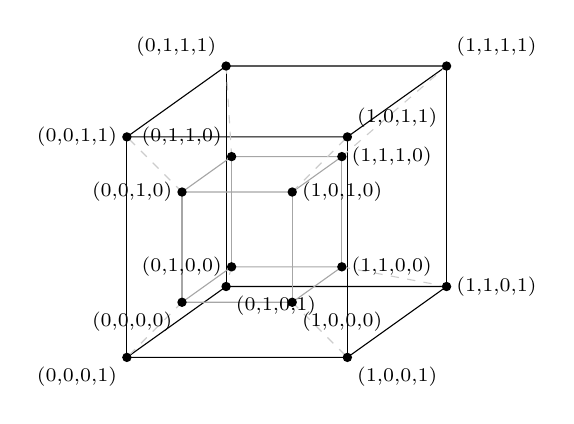
\begin{tikzpicture}[
        vertex/.style={circle,fill=black,inner sep=1.2pt},
        lbl/.style={font=\scriptsize},
        inner/.style={gray!70,thin},
        outer/.style={black,thin},
        conn/.style={gray!40,dashed,thin}
    ]
    

    \coordinate (i000) at (0.00,0.00);
    \coordinate (i100) at (1.40,0.00);
    \coordinate (i010) at (0.63,0.45);
    \coordinate (i110) at (2.03,0.45);
    \coordinate (i001) at (0.00,1.40);
    \coordinate (i101) at (1.40,1.40);
    \coordinate (i011) at (0.63,1.85);
    \coordinate (i111) at (2.03,1.85);
    

    \coordinate (o000) at (-0.70,-0.70);
    \coordinate (o100) at (2.10,-0.70);
    \coordinate (o010) at (0.56,0.20);
    \coordinate (o110) at (3.36,0.20);
    \coordinate (o001) at (-0.70,2.10);
    \coordinate (o101) at (2.10,2.10);
    \coordinate (o011) at (0.56,3.00);
    \coordinate (o111) at (3.36,3.00);
    

    \draw[outer] (o000)--(o100) (o100)--(o110) (o110)--(o010) (o010)--(o000);
    \draw[outer] (o001)--(o101) (o101)--(o111) (o111)--(o011) (o011)--(o001);
    \draw[outer] (o000)--(o001) (o100)--(o101) (o110)--(o111) (o010)--(o011);
    
    \draw[inner] (i000)--(i100) (i100)--(i110) (i110)--(i010) (i010)--(i000);
    \draw[inner] (i001)--(i101) (i101)--(i111) (i111)--(i011) (i011)--(i001);
    \draw[inner] (i000)--(i001) (i100)--(i101) (i110)--(i111) (i010)--(i011);
    
    \draw[conn] (i000)--(o000) (i100)--(o100) (i110)--(o110) (i010)--(o010);
    \draw[conn] (i001)--(o001) (i101)--(o101) (i111)--(o111) (i011)--(o011);
    

    \node[vertex] at (i000) {}; \node[lbl,below left]  at (i000) {(0,0,0,0)};
    \node[vertex] at (i100) {}; \node[lbl,below right] at (i100) {(1,0,0,0)};
    \node[vertex] at (i010) {}; \node[lbl,left]        at (i010) {(0,1,0,0)};
    \node[vertex] at (i110) {}; \node[lbl,right]       at (i110) {(1,1,0,0)};
    \node[vertex] at (i001) {}; \node[lbl,left]        at (i001) {(0,0,1,0)};
    \node[vertex] at (i101) {}; \node[lbl,right]       at (i101) {(1,0,1,0)};
    \node[vertex] at (i011) {}; \node[lbl,above left]  at (i011) {(0,1,1,0)};
    \node[vertex] at (i111) {}; \node[lbl, right] at (i111) {(1,1,1,0)};
    
    \node[vertex] at (o000) {}; \node[lbl,below left]  at (o000) {(0,0,0,1)};
    \node[vertex] at (o100) {}; \node[lbl,below right] at (o100) {(1,0,0,1)};
    \node[vertex] at (o010) {}; \node[lbl,below right] at (o010) {(0,1,0,1)};
    \node[vertex] at (o110) {}; \node[lbl,right]       at (o110) {(1,1,0,1)};
    \node[vertex] at (o001) {}; \node[lbl,left]        at (o001) {(0,0,1,1)};
    \node[vertex] at (o101) {}; \node[lbl,above right] at (o101) {(1,0,1,1)};
    \node[vertex] at (o011) {}; \node[lbl,above left]  at (o011) {(0,1,1,1)};
    \node[vertex] at (o111) {}; \node[lbl,above right] at (o111) {(1,1,1,1)};
    
    \end{tikzpicture}
    \end{center}
\color{teal} I genuinely wanna know how you have the patience to code this . . . cool stuff! \color{black}
\end{solution}
\begin{proof}
    Assume not. Then, there is a move for $N$ that $P$ cannot imitate by flipping the X Y Z bits. Let the vertex removed by $N$ be $A$ and its reflection be $B$. This means that there is at least one neighbor of $A$ that has not been removed till now, and all the neighbors of $B$ have been removed. 
    \newline
    \newline
    WLoG take $A=(0,0,0,1)$, $B=(1,1,1,1)$. The neighbors of $A$ are $(0,0,1,1)$, $(1,0,0,1)$, and $(0,1,0,1)$, while the neighbors $B$ are $(0,1,1,1)$, $(1,0,1,1)$, and $(1,1,0,1)$. We can notice that there is a one to one function(a reflection relation) between the three neighbors of $A$ and $B$. Thus, since all of $B$'s neighbors were removed, all of $A$'s neighbors should also have been removed. 
    \newline
    \newline
    Contradiction. Therefore $P$ can always imitate $N$'s movements and therefore can always win. \color{red}Great! This works.\color{black} \color{amethyst}Very nice proof\color{black}
\end{proof}
\item Prove by induction that every connected graph of order at least two has at least two vertices, $a$ and $b$, such that $G-a$ is connected, and $G-b$ is connected. 
\begin{proof}
    Let us use proof by induction. 
    \begin{enumerate}
        \item Base Case $n=2$. 
        \newline
        Both vertices act as $a$ and $b,$ and removing either one leaves a singular and connected vertex.
        \item Inductive Step. 
        \newline 
        \textbf{Assume we have a graph $G_k$ of order $k\geq2$ that is connected and containing vertices $a_k$ and $b_k$ such that $G-a_k$ and $G-b_k$ are connected.}
        \newline
        We add a new vertex $v_{k+1}$ to produce $G_{k+1}.$ \color{red}There's a subtle error here; you're effectively assuming that your order $k+1$ graph $G_{k+1}$ contains a vertex whose removal leaves the graph connected. This already assumes half of what you're trying to prove!!\color{black} We simply assign $v_{k+1}$ as $a_{k+1}$ (WLoG), and one of $a_k$ or $b_k$ as $b_{k+1}.$ This works because if $v_{k+1}$ is only connected to either $a_k$ or $b_k,$ we choose the other as $b_{k+1}.$
        
        
    \end{enumerate}
\end{proof}

\item \color{red}\textit{CHALLENGE. }\color{black} Assume the result of problem 5d is proven. Prove or disprove : Let $s$ be the number of stars in a game of cutthroat on a collection of stars. Let the number of petals on star $j=p_j$. Let $M=s+\sum_{j=1}^s(p_j-1)$. If $M$ is even, the collection is a $P$ game. If $M$ is odd, the collection is an $N$ game. 
\item \color{red}\textit{CHALLENGE. }\color{black} Is the petersen Graph $N$ or $P$? Make sure to prove your answer.  

We guess N. \color{red}That's rough, buddy.\color{black}

\item \color{blue}\textit{UNSOLVED. }\color{black} Tree Packing Conjecture made by Gyárfás: Any set of trees with $2,3,\dots,k$ vertices has an (edge=disjoint) packing into the complete graph on $k$ vertices.

\item \color{blue}\textit{SOLVED? }\color{black} How can one class be so awesome.  
\textbf{Answer. } Two conditions: have awesome people ($\checkmark$) and have an awesome subject ($\checkmark$).
\color{green} Very nice! Thank you for responding :) \color{black}

\item \color{blue}\textit{UNSOLVED. }\color{black} As $n\rightarrow\infty,$ does the pancake number $P_n$ approach $\frac{3}{2}n, \frac{1+\sqrt{5}}{2}n,$ or something else?


\color{teal} Hehehehehe, I am chuckling \color{black}
\begin{figure}[htbp]
    \centering
    
\includegraphics[width=0.75\linewidth]{yodaspat.png}
    \caption{\textit{\textbf{Pancakes}}}
    \label{fig:pancakes}
\end{figure}

\end{enumerate}

\color{amethyst}Nicely done overall!
\end{document}